\documentclass{standalone}
\usepackage{graphicx} % Required for inserting images
\usepackage{tikz}
\usetikzlibrary{positioning}
\usetikzlibrary{shapes,arrows} 
\newcommand{\sse}{\mathrm{ss}}
\newcommand{\re}{\mathrm{ref}}
\usepackage{amsmath, amsthm}
\usepackage{booktabs}
\usepackage{tabularx}
\usepackage{circuitikz}
\tikzstyle{block} = [draw, fill=blue!20, rectangle, minimum height=3em, minimum width=4em]
\tikzstyle{controller} = [draw, fill=red!20, rectangle, minimum height=3em, minimum width=4em]
\tikzstyle{sum} = [draw, fill=blue!20, circle, node distance=1cm]
\tikzstyle{input} = [coordinate]
\tikzstyle{output} = [coordinate]

\begin{document}
    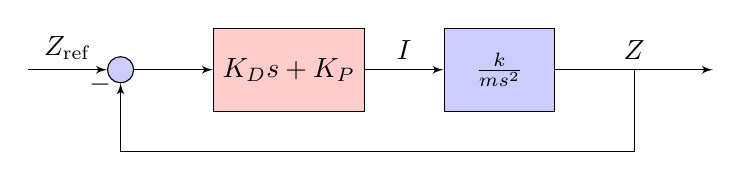
\begin{tikzpicture}[auto, >=latex']
        % Nodes
        \node [input] (input) {};
        \node [sum, right = 1cm of input] (sum) {};
        \node [controller, right = 1cm of sum] (system) {$K_D s + K_P$};
        \node [block, right = 1cm of system] (system2) {$\frac{k}{ms^2}$};
        \node [output, right = 2cm of system2] (output) {};
        \node [input, below = 0.5cm of system] (m) {};
        % Arrows
        \draw [draw,->] (input) -- node {$Z_\re$} (sum);
        \draw [->] (sum) -- node {} (system);
        \draw [->] (system) -- node {$I$} (system2);
        \draw [->] (system2) -- node (y) {$Z$}(output);
        \draw [-] (y) |- (m) {} ;
        \draw [->] (m) -| node[pos=0.99] {$-$}  node [near end] {} (sum);
    \end{tikzpicture}  
    % \end{lateximage}% NEW
    % \caption{Proportional-derivative control.}
\end{document}